\begin{wrapfigure}{r}[5pt]{0.4\textwidth}
	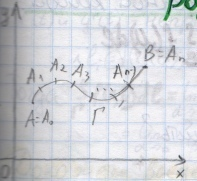
\includegraphics[scale=0.7]{int1.jpg}
\end{wrapfigure}

Пусть в $xOy$ задана спрямляемая кривая, т.е. кривая, у которой есть длина.
И пусть есть функция $f(x,y)$, которая определена на $\Gamma$ (или на Д: Д > $\Gamma$).


Разобъём кривую AB точками $A_i$.
Возьмём $\forall(M;\in \Gamma)$.
Пусть $(\zeta_i;\eta_i )$ --- координаты $M_i$.
Найдем $(\zeta_i;\eta_i )$ и составим сумму: $S_n = \sum^{n}_{i=1} {f(\zeta_i;\eta_i )}_n l_i$

Аналогично можно сделать и в случае если кривая замкнута. Только тогда надо указать начало и направление.

\opred
Если $\exists (\lim\limits_{\alpha \rightarrow 0}(S_n = I) [I \ne 0]$, где $\alpha = \max \triangle l_i$, $S_n = S_n = \sum^{n}_{i=1} {f(\zeta_i;\eta_i )}_n l_i$,
причем I не зависит ни от способа разбиения I на части, ни от выбранных точек $M_i$, то I --- это криволинейный интеграл от $f(x,y)$, взятый по кривой $\Gamma$.
\opred


$$ I = \int\limits_{\Gamma}f(x,y)dxdy = \int\limits_{\Gamma}f(M)dl$$.


Если вернуться к массе нити, то очевидно, что $m=\int\limits{AB}\varrho(M)dl$.

Аналогично можно рассматривать интеграл и по пространственной кривой:

\begin{wrapfigure}{r}[5pt]{0.4\textwidth}
	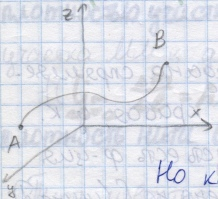
\includegraphics[scale=0.7]{int2.jpg}
\end{wrapfigure}

$\int\limits_{AB}f(x,y,z)dl = \int\limits_{AB}f(M)dl$.

